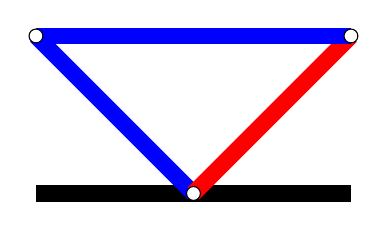
\begin{tikzpicture}
  % Styles tuned to match the visual appearance
  \tikzset{
    hacken node/.style={draw,circle,fill=white,inner sep=0pt,minimum size=5pt},
    hacken line/.style={line width=6pt,line cap=butt}
  }

  % Key coordinates
  \coordinate (B) at (2,0);  % bottom center
  \coordinate (L) at (0,2);  % top left
  \coordinate (R) at (4,2);  % top right

  % Ground (black)
  \draw[hacken line,black] (0,0) -- (4,0);

  % Edges
  \draw[hacken line,blue] (B) -- (L);
  \draw[hacken line,red]  (B) -- (R);
  \draw[hacken line,blue] (L) -- (R);

  % Nodes (drawn last so they appear on top of edges)
  \node[hacken node] at (B) {};
  \node[hacken node] at (L) {};
  \node[hacken node] at (R) {};
\end{tikzpicture}